\documentclass{article}
\usepackage{gensymb}
\usepackage{float}
\usepackage{graphicx}
\usepackage{minted}
\usepackage{amsmath}
\usepackage{pdfpages}
\usepackage{geometry}
\usepackage{hyperref}
\hypersetup{
    colorlinks=true,
    linkcolor=black,
    filecolor=magenta,      
    urlcolor=cyan,
    }
\geometry{margin = 1in}

\begin{document}
    \begin{titlepage}
        \centering
        \vspace{4cm}
        {\scshape\Huge Guía Práctica 1 \par}
        \vspace{3cm}
        {\itshape\Large Diseño Digital Avanzado \par}
        \vfill
        {\Large Mathias Sebastian Garcia\par}
        \vfill
        {\Large \today\par}
    \end{titlepage}

    \tableofcontents

    \newpage
    \section{Ejercicio 1}
    Código:
    \inputminted[fontsize=\scriptsize]{systemverilog}{../sum_accumulator/rtl/sum_accumulator.sv}

    Se realizaron 7 TCs utilizando cocotb, para no sobrecargar el archivo, se encuentran en \href{https://github.com/msebgarcia/DDA2024/tree/main/GP01/sum_accumulator/tb}{github}. Los mismos consisten en:
    \begin{itemize}
        \item TC001: Entrada constante con el selector en 2
        \item TC002: Entrada constante con el selector en 0
        \item TC003: Entrada constante con el selector en 1
        \item TC004: Ambas entradas en 1 con el selector en 1
        \item TC005: Cambio en las entradas de dato con selector constante
        \item TC006: Cambio en todas las entradas
        \item TC007: Reset y recuperación
    \end{itemize}
    El archivo \href{https://github.com/msebgarcia/DDA2024/blob/main/GP01/sum_accumulator/tb/test_module.py}{test\_module.py} contiene los TCs y en \href{https://github.com/msebgarcia/DDA2024/blob/main/GP01/sum_accumulator/tb/model.py}{model.py} se encuentra el modelado del RTL. Asimismo, se subió el .vcd donde se dumpearon las señales.
    \\
    Teniendo en cuenta que el acumulador suma de a 2 y la salida es de 6 bits, cuyo valor de cuenta máximo es 63, se necesitan 32 clocks para que produzca overflow.

    \newpage
    \section{Ejercicio 2}
    Código:
    \inputminted[fontsize=\scriptsize]{systemverilog}{../arith_operator/rtl/arith_operator.sv}

    Se realizaron 5 TCs, que se pueden encontrar en este \href{https://github.com/msebgarcia/DDA2024/blob/main/GP01/arith_operator/tb/test_module.py}{link de github}, utilizando cocotb al igual que en el inciso anterior:
    \begin{itemize}
        \item TC001: Suma con datos de entrada aleatorios
        \item TC002: Resta con datos de entrada aleatorios
        \item TC003: Operación And  con datos de entrada aleatorios
        \item TC004: Operación Or con datos de entrada aleatorios
        \item TC005: Randomización de operación y datos de entrada
    \end{itemize}
    En este caso, tanto el modelo del RTL como los TCs se colocaron en el mismo archivo por simplicidad. También se subió el .vcd donde se dumpearon las señales.
    
    \newpage
    \section{Ejercicio 3}
    \begin{center}
        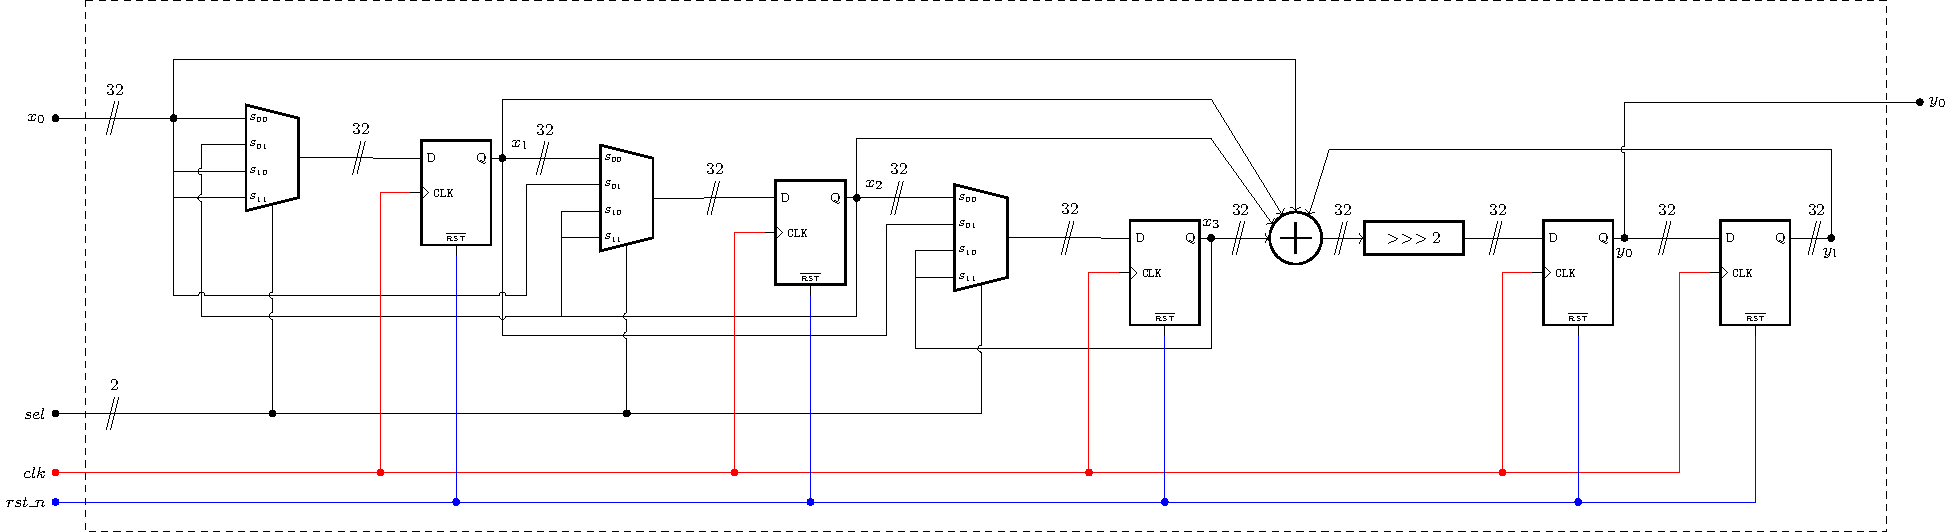
\includegraphics[angle=90, scale=.65]{../test_module/architecture.pdf}
    \end{center}
     
    \newpage
    \section{Ejercicio 4}
    \subsection{Arquitectura}
    \begin{center}
        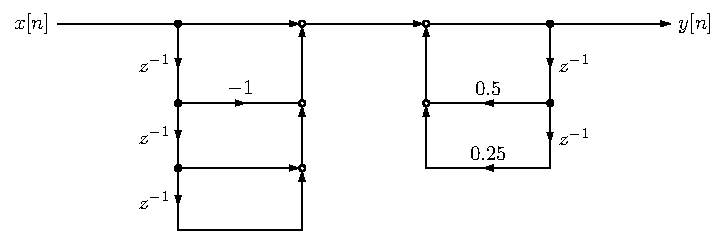
\includegraphics[width=\linewidth]{../iir_filter/draw/draw.pdf}
    \end{center}

    \subsection{Cálculo de la cantidad de bits de salida}
    Se consideró que las 4 muestras en X podían tener los valores límites, es decir, -128 y 127. De donde se obtiene un mínimo de $4\cdot(-128) = -512$ y un máximo de $4\cdot127 = 508$.\\
    Para el caso de las muestras en Y se tuvieron en cuenta los extremos considerados previamente, de donde se obtuvo: $0.75\cdot(-512) = -384$ y $0.75\cdot508 = 381$.\\
    A partir de estos extremos, se calculó el rango:
    \[
        rango =
        \begin{cases}
            Min = -512-384 = -896\\
            Max = 508+381 = 889\\
            Total = 889 - (-896) + 1 = 1786
        \end{cases}
    \]
    Para representar dicho rango se requieren 11 bits.

    \subsection{Testcases}
    Se plantearon 6 TCs, los cuales son:
    \begin{itemize}
        \item TC001: Entrada constante
        \item TC002: Cambio aleatorio en la entrada cada cinco clocks
        \item TC003: Onda senoidal de 50kHz
        \item TC004: Onda senoidal de 1MHz
        \item TC005: Onda senoidal de 10MHz
        \item TC006: Reset y recuperación con una onda cuadrada
    \end{itemize}
    Los mismos se pueden encontrar en \href{https://github.com/msebgarcia/DDA2024/tree/main/GP01/iir_filter/tb}{github}, estando los TCs en el archivo \href{https://github.com/msebgarcia/DDA2024/blob/main/GP01/iir_filter/tb/test_module.py}{test\_module.py} y el modelo del RTL en \href{https://github.com/msebgarcia/DDA2024/blob/main/GP01/iir_filter/tb/model.py}{model.py}. Al igual que en los ejercicios previos, se cargó el .vcd con el dump de las señales.

    \newpage
    \subsection{Código}
    \inputminted[fontsize=\scriptsize]{systemverilog}{../iir_filter/rtl/iir_filter.sv}
 
\end{document}
